\chapter{Cristaux II~: solides ioniques, covalents et moléculaires}\label{ch:b1:crystals-ionic-covalent}

Le sel de cuisine, broyé, se casse en minuscules cubes~; le diamant est
le matériau naturel le plus dur, et pourtant le graphite, fait des mêmes
atomes de carbone, est assez tendre pour qu'on écrive avec~; la glace
flotte sur l'eau. Tous sont des \omterm{def:b1:crystals-metals:crystal}{cristaux}, mais leurs particules sont
maintenues ensemble de façons différentes~: les ions par attraction
électrostatique, les atomes par des \omterm{def:b1:lewis-resonance-vsepr:lewis}{liaisons covalentes}, les molécules
par les interactions intermoléculaires du
\cref{ch:b1:intermolecular-forces-solvents}. Ce chapitre applique la
géométrie des \omterm{def:b1:crystals-metals:lattice}{mailles} du chapitre précédent à ces trois familles de
solides, et explique, à partir de la taille des ions, pourquoi le
chlorure de sodium et le chlorure de césium adoptent des structures
différentes.

\begin{recall}
La \omterm{def:b1:crystals-metals:multiplicity}{multiplicité} d'une \omterm{def:b1:crystals-metals:lattice}{maille}, la \omterm{def:b1:crystals-metals:coordination}{coordinence} et la \omterm{def:b1:crystals-metals:compactness}{compacité}, ainsi que
les \omterm{def:b1:crystals-metals:site}{sites octaédriques} et tétraédriques du \omterm{def:b1:crystals-metals:lattice}{réseau} \omterm{def:b1:crystals-metals:packings}{cubique à faces
centrées}, ont été définis au \cref{ch:b1:crystals-metals}~; la masse
volumique d'un \omterm{def:b1:crystals-metals:crystal}{cristal} vaut $\rho = ZM/(N_A V)$
(\cref{prop:b1:crystals-metals:density}). Les \omterm{def:b1:periodicity:radius}{rayons ioniques} ont été
introduits à la \cref{def:b1:periodicity:radius}.
\end{recall}

\section{Cristaux ioniques et rapport des rayons}

\begin{definition}[Cristal ionique]\label{def:b1:crystals-ionic-covalent:ionic-crystal}
Un \emph{cristal ionique}\index{cristal ionique} est un \omterm{def:b1:crystals-metals:crystal}{cristal} de
cations et d'anions maintenus ensemble par attraction électrostatique.
Chaque ion est entouré d'ions de charge opposée~; le \omterm{def:b1:crystals-metals:crystal}{cristal} est
électriquement neutre, si bien que les nombres de cations et d'anions
d'une \omterm{def:b1:crystals-metals:lattice}{maille} sont dans le rapport de la formule.
\end{definition}

\begin{proposition}[Propriétés des cristaux ioniques]\label{prop:b1:crystals-ionic-covalent:ionic-properties}
Les \omterm{def:b1:crystals-ionic-covalent:ionic-crystal}{cristaux ioniques} sont durs mais cassants (le glissement d'un plan
met face à face des ions de même signe, et le \omterm{def:b1:crystals-metals:crystal}{cristal} se clive), ont des
températures de fusion élevées, ne conduisent pas à l'état solide mais
conduisent fondus ou dissous, et se dissolvent dans les \omterm{def:b1:intermolecular-forces-solvents:solvent-classes}{solvants
polaires} de forte permittivité.
\end{proposition}
\admitted

\begin{definition}[Rapport des rayons]\label{def:b1:crystals-ionic-covalent:radius-ratio}
Dans un \omterm{def:b1:crystals-ionic-covalent:ionic-crystal}{cristal ionique} formé d'un cation de rayon $r_+$ et d'un anion
de rayon $r_-$, le \emph{rapport des rayons}\index{rapport des rayons} est $x = r_+/r_-$
(en général $x < 1$, les cations étant plus petits que les anions).
\end{definition}

\begin{proposition}[La règle du rapport des rayons]\label{prop:b1:crystals-ionic-covalent:rule}
Dans le modèle des sphères dures, une structure dans laquelle chaque
cation touche $n$ anions n'est stable que si les anions ne se touchent
pas entre eux, ce qui exige que $x$ dépasse une limite fixée par la
géométrie~: $x \ge \sqrt3 - 1
\approx 0.732$ pour 8 voisins (cube), $x \ge \sqrt2 - 1 \approx 0.414$
pour 6 (octaèdre), $x \ge \sqrt{3/2} - 1 \approx 0.225$ pour 4
(tétraèdre). La structure adoptée est celle de plus haute \omterm{def:b1:crystals-metals:coordination}{coordinence}
que permet $x$.
\end{proposition}

\begin{proof}
Le cation se loge dans le vide ménagé entre $n$ anions qui sont à son
contact. À la limite, les anions se touchent aussi entre eux. Cube~: les
anions occupent les sommets d'un cube d'arête $2r_-$ et le cation son
centre, donc $r_+ +
r_- = \sqrt3\,r_-$. Octaèdre~: quatre anions en carré de côté $2r_-$, le
cation en son centre, $r_+ + r_- = \sqrt2\,r_-$. Tétraèdre~: les anions
occupent des sommets alternés d'un cube d'arête $\sqrt2\,r_-$, le cation
le centre, $r_+ + r_- = \frac{\sqrt3}{2}\sqrt2\,r_- = \sqrt{3/2}\,r_-$.
La division par $r_-$ donne les limites. Sous la limite, le cation
ballotte dans un vide trop grand pour lui~: les anions se repoussent sans
que l'attraction augmente, et une \omterm{def:b1:crystals-metals:coordination}{coordinence} plus faible, avec un vide
plus petit, est préférée.
\end{proof}

\begin{omfigure}
\begin{tikzpicture}[font=\small, >={Stealth}]
  \draw[->, thick] (0,0) -- (12.4,0) node[right] {$x = r_+/r_-$};
  \foreach \x/\l in {0/0, 2.7/0.225, 4.97/0.414, 8.78/0.732, 12/1} {
    \draw (\x,0.12) -- (\x,-0.12) node[below] {\l};
  }
  \fill[omDef!15] (2.7,0.2) rectangle (4.97,1.0);
  \fill[omProp!15] (4.97,0.2) rectangle (8.78,1.0);
  \fill[omThm!15] (8.78,0.2) rectangle (12,1.0);
  \node[align=center] at (3.83,0.6) {4: ZnS};
  \node[align=center] at (6.87,0.6) {6: NaCl};
  \node[align=center] at (10.4,0.6) {8: CsCl};
  \foreach \x/\l in {3.91/\ce{ZnS}, 6.76/\ce{NaCl}, 10.08/\ce{RbCl}, 11.54/\ce{CsCl}} {
    \draw[omExo, thick] (\x,-0.55) -- (\x,-0.95);
    \node[below, omExo] at (\x,-0.95) {\l};
  }
\end{tikzpicture}

{\small La règle du \omterm{def:b1:crystals-ionic-covalent:radius-ratio}{rapport des rayons}~: la \omterm{def:b1:crystals-metals:coordination}{coordinence} du cation
permise par $x$, et les rapports mesurés de quatre sels (rayons de
Shannon). Le chlorure de rubidium, à 0.84, devrait être du type
\ce{CsCl} mais adopte le type \ce{NaCl}~: la règle est un guide, non une
loi (\cref{exo:b1:crystals-ionic-covalent:12}).}
% ledger: rion:Zn2+IV, rion:S2-VI, rion:Na+VI, rion:Cl-VI, rion:Rb+VI,
% rion:Cs+VIII
\end{omfigure}

\section{Quatre types structuraux}

\begin{definition}[Types structuraux]\label{def:b1:crystals-ionic-covalent:structure-type}
Les \omterm{def:b1:crystals-ionic-covalent:ionic-crystal}{cristaux ioniques} se classent en quelques types structuraux, qui
portent le nom d'un composé représentatif~:
\begin{itemize}
  \item le \emph{type chlorure de césium}\index{type chlorure de cesium@type chlorure de césium}~: les anions
        aux sommets d'un cube, le cation en son centre (8:8)~;
  \item le \emph{type sel gemme}\index{type sel gemme} (type chlorure de
        sodium)~: les anions sur un \omterm{def:b1:crystals-metals:lattice}{réseau} CFC, les cations dans tous ses
        \omterm{def:b1:crystals-metals:site}{sites octaédriques} (6:6)~;
  \item le \emph{type blende}\index{type blende}~: les anions sur un
        \omterm{def:b1:crystals-metals:lattice}{réseau} CFC, les cations dans la moitié de ses \omterm{def:b1:crystals-metals:site}{sites tétraédriques},
        un sur deux en alternance (4:4)~;
  \item le \emph{type fluorine}\index{type fluorine}~: les cations sur un
        \omterm{def:b1:crystals-metals:lattice}{réseau} CFC, les anions dans tous ses \omterm{def:b1:crystals-metals:site}{sites tétraédriques} (8:4),
        formule \ce{MX2}~; dans le \emph{type antifluorine}\index{type antifluorine}
        les rôles sont échangés (\ce{Li2O}, 4:8).
\end{itemize}
Le couple de nombres donne la \omterm{def:b1:crystals-metals:coordination}{coordinence} du cation et celle de l'anion.
\end{definition}

\begin{omfigure}
\tdplotsetmaincoords{60}{100}
\begin{tikzpicture}[tdplot_main_coords, font=\small]
  \pic {omcubeo={3}};
    \node[aX={green!55!black}{6.5mm}] at (0,0,0) {};
  \node[aX={violet!70}{3.8mm}] at (0,1.5,0) {};
  \node[aX={green!55!black}{6.5mm}] at (0,3,0) {};
  \node[aX={violet!70}{3.8mm}] at (0,0,1.5) {};
  \node[aX={green!55!black}{6.5mm}] at (0,1.5,1.5) {};
  \node[aX={violet!70}{3.8mm}] at (0,3,1.5) {};
  \node[aX={violet!70}{3.8mm}] at (1.5,0,0) {};
  \node[aX={green!55!black}{6.5mm}] at (0,0,3) {};
  \node[aX={green!55!black}{6.5mm}] at (1.5,1.5,0) {};
  \node[aX={violet!70}{3.8mm}] at (0,1.5,3) {};
  \node[aX={violet!70}{3.8mm}] at (1.5,3,0) {};
  \node[aX={green!55!black}{6.5mm}] at (0,3,3) {};
  \node[aX={green!55!black}{6.5mm}] at (1.5,0,1.5) {};
  \node[aX={violet!70}{3.8mm}] at (1.5,1.5,1.5) {};
  \node[aX={green!55!black}{6.5mm}] at (1.5,3,1.5) {};
  \node[aX={green!55!black}{6.5mm}] at (3,0,0) {};
  \node[aX={violet!70}{3.8mm}] at (1.5,0,3) {};
  \node[aX={violet!70}{3.8mm}] at (3,1.5,0) {};
  \node[aX={green!55!black}{6.5mm}] at (1.5,1.5,3) {};
  \node[aX={green!55!black}{6.5mm}] at (3,3,0) {};
  \node[aX={violet!70}{3.8mm}] at (1.5,3,3) {};
  \node[aX={violet!70}{3.8mm}] at (3,0,1.5) {};
  \node[aX={green!55!black}{6.5mm}] at (3,1.5,1.5) {};
  \node[aX={violet!70}{3.8mm}] at (3,3,1.5) {};
  \node[aX={green!55!black}{6.5mm}] at (3,0,3) {};
  \node[aX={violet!70}{3.8mm}] at (3,1.5,3) {};
  \node[aX={green!55!black}{6.5mm}] at (3,3,3) {};
  \node at (1.5,1.5,-1.75) {\ce{NaCl} (sel gemme)};
\end{tikzpicture}
\hspace{1cm}
\begin{tikzpicture}[tdplot_main_coords, font=\small]
  \pic {omcubeo={3}};
    \node[aX={green!55!black}{6.5mm}] at (0,0,0) {};
  \node[aX={green!55!black}{6.5mm}] at (0,3,0) {};
  \node[aX={green!55!black}{6.5mm}] at (0,0,3) {};
  \node[aX={green!55!black}{6.5mm}] at (0,3,3) {};
  \node[aX={blue!60}{7mm}] at (1.5,1.5,1.5) {};
  \node[aX={green!55!black}{6.5mm}] at (3,0,0) {};
  \node[aX={green!55!black}{6.5mm}] at (3,3,0) {};
  \node[aX={green!55!black}{6.5mm}] at (3,0,3) {};
  \node[aX={green!55!black}{6.5mm}] at (3,3,3) {};
  \node at (1.5,1.5,-1.75) {\ce{CsCl}};
\end{tikzpicture}

{\small À gauche~: la \omterm{def:b1:crystals-metals:lattice}{maille} du sel gemme, \ce{Cl-} (en vert) sur un
\omterm{def:b1:crystals-metals:lattice}{réseau} CFC, \ce{Na+} (en violet) dans tous les \omterm{def:b1:crystals-metals:site}{sites octaédriques}. À
droite~: la \omterm{def:b1:crystals-metals:lattice}{maille} du chlorure de césium, \ce{Cl-} aux sommets, \ce{Cs+}
(en bleu) au centre. Ions dessinés plus petits qu'au contact.}
\end{omfigure}

\begin{proposition}[Types sel gemme et chlorure de césium]\label{prop:b1:crystals-ionic-covalent:nacl-cscl}
Dans le \omterm{def:b1:crystals-ionic-covalent:structure-type}{type sel gemme}, $Z = 4$ unités formulaires par \omterm{def:b1:crystals-metals:lattice}{maille}, les ions
sont tangents le long d'une arête, $a = 2(r_+ + r_-)$, et la structure
exige $\sqrt2 - 1
\le x$. Dans le \omterm{def:b1:crystals-ionic-covalent:structure-type}{type chlorure de césium}, $Z = 1$, les ions sont tangents
le long de la grande diagonale, $a\sqrt3 = 2(r_+ + r_-)$, et la
structure exige $x \ge \sqrt3 - 1$.
\end{proposition}

\begin{proof}
Sel gemme~: les anions du \omterm{def:b1:crystals-metals:lattice}{réseau} CFC sont au nombre de $4$, les cations
des 4 \omterm{def:b1:crystals-metals:site}{sites octaédriques} $1 + 12 \times \frac14 = 4$. Le long d'une
arête se suivent, au contact, un anion, un cation et un anion. Les
anions ne s'interpénètrent pas si la diagonale de face, qui porte trois
anions dont deux au plus se touchent, vérifie $a\sqrt2 \ge 4r_-$,
c'est-à-dire $2(r_+ + r_-)\sqrt2 \ge
4r_-$, soit $x \ge \sqrt2 - 1$. Chlorure de césium~: $8 \times \frac18 = 1$
anion et 1 cation~; sur la grande diagonale, anion, cation, anion au
contact~; les anions ne s'interpénètrent pas le long d'une arête si
$a \ge 2r_-$, c'est-à-dire
$2(r_+ + r_-)/\sqrt3 \ge 2r_-$, soit $x \ge \sqrt3 - 1$.
\end{proof}

\begin{example}[Chlorure de sodium et chlorure de césium]\label{ex:b1:crystals-ionic-covalent:nacl}
Le chlorure de sodium a $a = \qty{564.1}{pm}$~: $r_+ + r_- = a/2 =
\qty{282.0}{pm}$, contre $102 + 181 = \qty{283}{pm}$ d'après les rayons
de Shannon~; $x = 102/181 = 0.56$, dans le domaine octaédrique. Sa masse
volumique vaut
$\rho = 4 \times 58.44/(6.022 \times 10^{23} \times (5.641 \times
10^{-8})^3) = \qty{2.16}{g/cm^3}$, pour \qty{2.17}{g/cm^3} mesurés. Le
chlorure de césium a $a = \qty{412.3}{pm}$~: $r_+ + r_- = a\sqrt3/2 =
\qty{357.1}{pm}$, et $x = 174/181 = 0.96$, dans le domaine cubique.
% ledger: lat:NaCl, rion:Na+VI, rion:Cl-VI, rho:NaCl, lat:CsCl,
% rion:Cs+VIII
\end{example}

\begin{omfigure}
\begin{minipage}[b]{0.31\linewidth}\centering
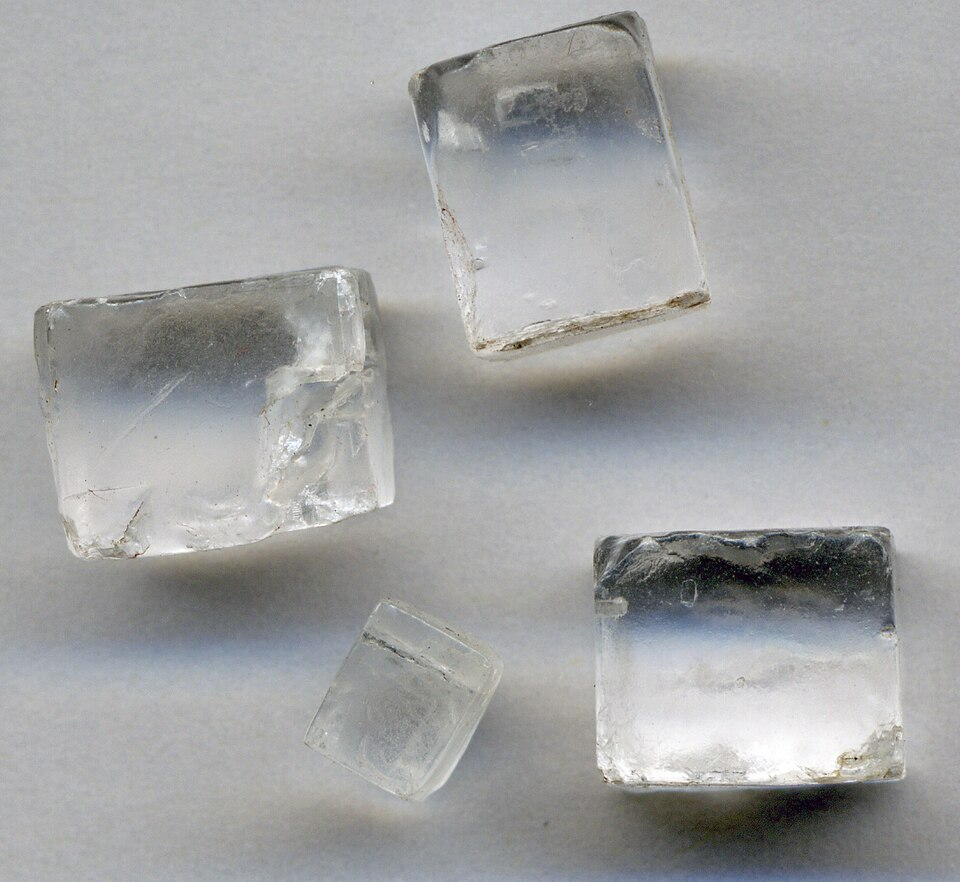
\includegraphics[width=\linewidth]{images/book2/halite.jpg}

{\small \omterm{def:b1:crystals-metals:crystal}{Cristaux} de halite (sel gemme). Photo~: James St. John, CC BY 2.0.}
\end{minipage}\hfill
\begin{minipage}[b]{0.31\linewidth}\centering
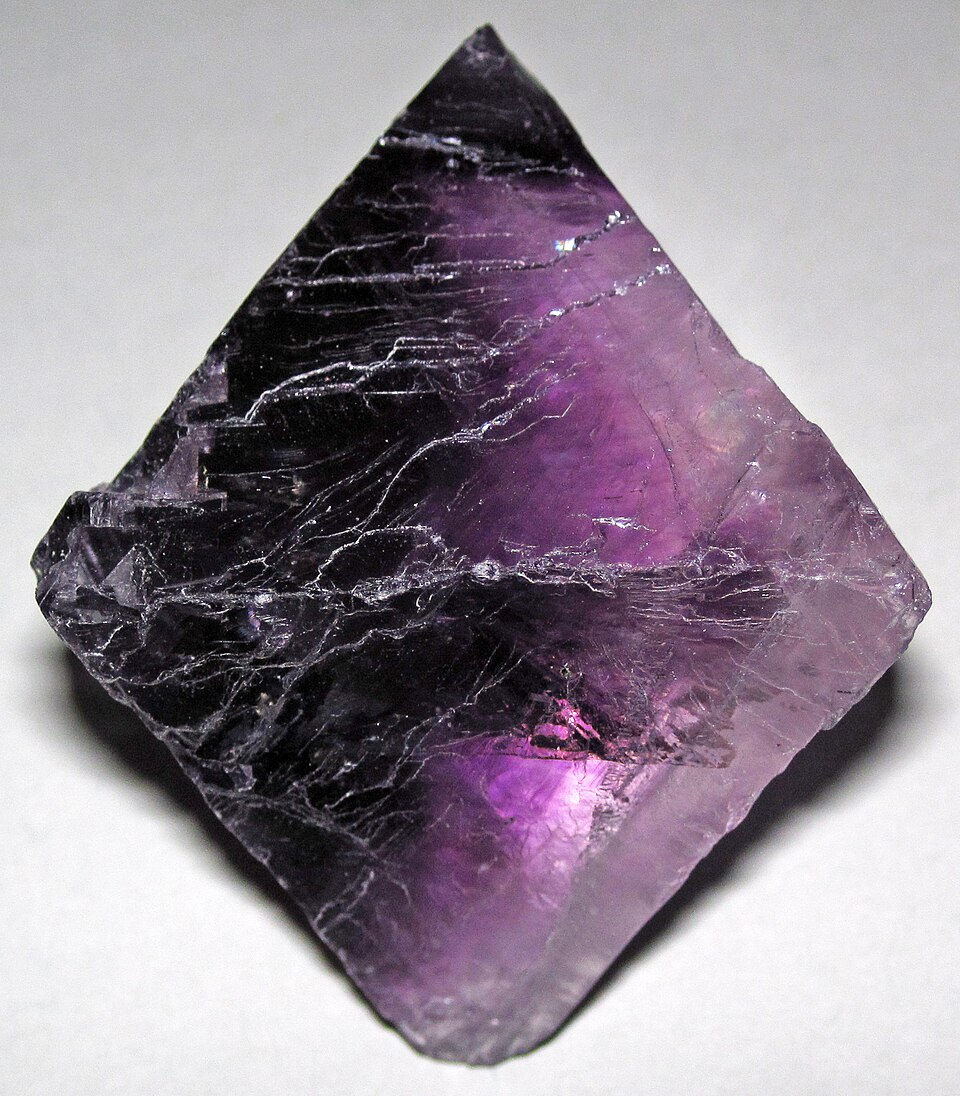
\includegraphics[width=0.85\linewidth]{images/book2/fluorite.jpg}

{\small Fluorine, \ce{CaF2}. Photo~: James St. John, CC BY 2.0.}
\end{minipage}\hfill
\begin{minipage}[b]{0.31\linewidth}\centering
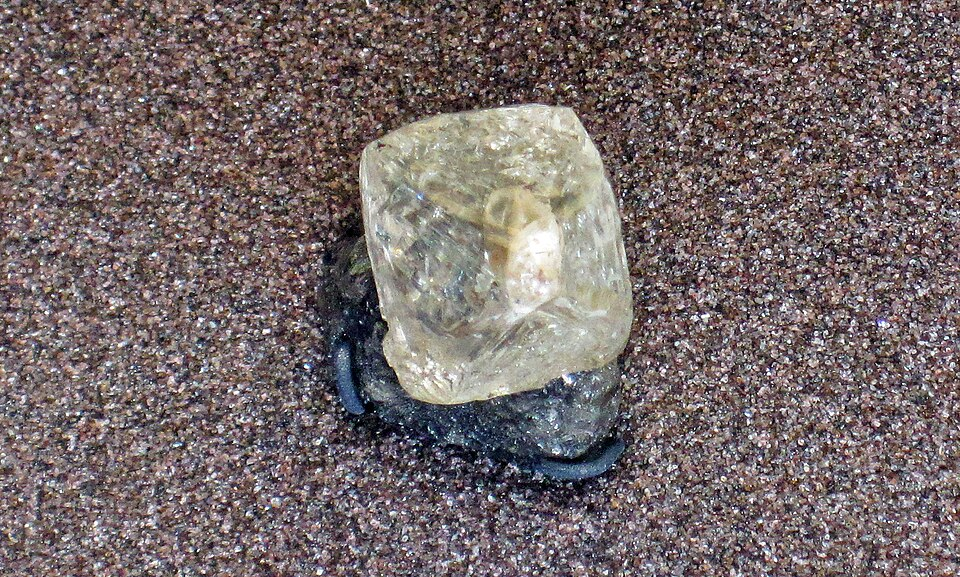
\includegraphics[width=\linewidth]{images/book2/diamond.jpg}

{\small Un octaèdre de diamant brut. Photo~: James St. John, CC BY 2.0.}
\end{minipage}
\end{omfigure}

\begin{proposition}[Types blende et fluorine]\label{prop:b1:crystals-ionic-covalent:zns-caf2}
Dans le \omterm{def:b1:crystals-ionic-covalent:structure-type}{type blende}, $Z = 4$, chaque ion est entouré de quatre ions de
l'autre sorte aux sommets d'un tétraèdre, et les ions sont tangents le
long d'un quart de la grande diagonale~: $a\sqrt3/4 = r_+ + r_-$. Dans
le \omterm{def:b1:crystals-ionic-covalent:structure-type}{type fluorine}, $Z = 4$ unités \ce{CaF2}, chaque cation a 8 anions
voisins (un cube), chaque anion 4 cations voisins (un tétraèdre), et de
nouveau $a\sqrt3/4 =
r_+ + r_-$.
\end{proposition}

\begin{proof}
Blende~: 4 anions sur le \omterm{def:b1:crystals-metals:lattice}{réseau} CFC et 4 cations dans la moitié des 8
\omterm{def:b1:crystals-metals:site}{sites tétraédriques}. Un \omterm{def:b1:crystals-metals:site}{site tétraédrique} en $(\frac a4,\frac a4,\frac a4)$
se trouve à $\frac{a\sqrt3}{4}$ de ses quatre anions. Fluorine~: 4
cations et 8 anions dans tous les \omterm{def:b1:crystals-metals:site}{sites tétraédriques}, rapport $1:2$.
Les 8 anions intérieurs à la \omterm{def:b1:crystals-metals:lattice}{maille} forment un cube d'arête $a/2$~;
dans le \omterm{def:b1:crystals-metals:crystal}{cristal}, les anions forment ainsi des cubes dont un sur deux
contient un cation en son centre~; un anion a ses 4 cations voisins à
$\frac{a\sqrt3}{4}$.
\end{proof}

\begin{omfigure}
\tdplotsetmaincoords{60}{100}
\begin{tikzpicture}[tdplot_main_coords, font=\small]
  \pic {omcubeo={3}};
  \begin{scope}[on background layer]
    \draw[black!45, line width=1.2pt] (0.75,0.75,2.25) -- (0,0,3) (0.75,0.75,2.25) -- (0,1.5,1.5) (0.75,0.75,2.25) -- (1.5,0,1.5) (0.75,0.75,2.25) -- (1.5,1.5,3) (0.75,2.25,0.75) -- (0,1.5,1.5) (0.75,2.25,0.75) -- (0,3,0) (0.75,2.25,0.75) -- (1.5,1.5,0) (0.75,2.25,0.75) -- (1.5,3,1.5) (2.25,0.75,0.75) -- (1.5,0,1.5) (2.25,0.75,0.75) -- (1.5,1.5,0) (2.25,0.75,0.75) -- (3,0,0) (2.25,0.75,0.75) -- (3,1.5,1.5) (2.25,2.25,2.25) -- (1.5,1.5,3) (2.25,2.25,2.25) -- (1.5,3,1.5) (2.25,2.25,2.25) -- (3,1.5,1.5) (2.25,2.25,2.25) -- (3,3,3);
  \end{scope}
    \node[aX={yellow!75!orange}{6mm}] at (0,0,0) {};
  \node[aX={yellow!75!orange}{6mm}] at (0,3,0) {};
  \node[aX={yellow!75!orange}{6mm}] at (0,1.5,1.5) {};
  \node[aX={gray!60}{3.6mm}] at (0.75,2.25,0.75) {};
  \node[aX={yellow!75!orange}{6mm}] at (0,0,3) {};
  \node[aX={yellow!75!orange}{6mm}] at (1.5,1.5,0) {};
  \node[aX={gray!60}{3.6mm}] at (0.75,0.75,2.25) {};
  \node[aX={yellow!75!orange}{6mm}] at (0,3,3) {};
  \node[aX={yellow!75!orange}{6mm}] at (1.5,0,1.5) {};
  \node[aX={gray!60}{3.6mm}] at (2.25,0.75,0.75) {};
  \node[aX={yellow!75!orange}{6mm}] at (1.5,3,1.5) {};
  \node[aX={yellow!75!orange}{6mm}] at (3,0,0) {};
  \node[aX={yellow!75!orange}{6mm}] at (1.5,1.5,3) {};
  \node[aX={yellow!75!orange}{6mm}] at (3,3,0) {};
  \node[aX={gray!60}{3.6mm}] at (2.25,2.25,2.25) {};
  \node[aX={yellow!75!orange}{6mm}] at (3,1.5,1.5) {};
  \node[aX={yellow!75!orange}{6mm}] at (3,0,3) {};
  \node[aX={yellow!75!orange}{6mm}] at (3,3,3) {};
  \node at (1.5,1.5,-1.75) {\ce{ZnS} (blende)};
\end{tikzpicture}
\hspace{1cm}
\begin{tikzpicture}[tdplot_main_coords, font=\small]
  \pic {omcubeo={3}};
    \node[aX={green!35!gray}{4.4mm}] at (0,0,0) {};
  \node[aX={green!35!gray}{4.4mm}] at (0,3,0) {};
  \node[aX={green!35!gray}{4.4mm}] at (0,1.5,1.5) {};
  \node[aX={green!45!yellow}{5.0mm}] at (0.75,0.75,0.75) {};
  \node[aX={green!45!yellow}{5.0mm}] at (0.75,2.25,0.75) {};
  \node[aX={green!35!gray}{4.4mm}] at (0,0,3) {};
  \node[aX={green!35!gray}{4.4mm}] at (1.5,1.5,0) {};
  \node[aX={green!45!yellow}{5.0mm}] at (0.75,0.75,2.25) {};
  \node[aX={green!35!gray}{4.4mm}] at (0,3,3) {};
  \node[aX={green!35!gray}{4.4mm}] at (1.5,0,1.5) {};
  \node[aX={green!45!yellow}{5.0mm}] at (0.75,2.25,2.25) {};
  \node[aX={green!45!yellow}{5.0mm}] at (2.25,0.75,0.75) {};
  \node[aX={green!35!gray}{4.4mm}] at (1.5,3,1.5) {};
  \node[aX={green!35!gray}{4.4mm}] at (3,0,0) {};
  \node[aX={green!45!yellow}{5.0mm}] at (2.25,2.25,0.75) {};
  \node[aX={green!35!gray}{4.4mm}] at (1.5,1.5,3) {};
  \node[aX={green!35!gray}{4.4mm}] at (3,3,0) {};
  \node[aX={green!45!yellow}{5.0mm}] at (2.25,0.75,2.25) {};
  \node[aX={green!45!yellow}{5.0mm}] at (2.25,2.25,2.25) {};
  \node[aX={green!35!gray}{4.4mm}] at (3,1.5,1.5) {};
  \node[aX={green!35!gray}{4.4mm}] at (3,0,3) {};
  \node[aX={green!35!gray}{4.4mm}] at (3,3,3) {};
  \node at (1.5,1.5,-1.75) {\ce{CaF2} (fluorine)};
\end{tikzpicture}

{\small À gauche~: la blende, \ce{S^{2-}} (en jaune) sur un \omterm{def:b1:crystals-metals:lattice}{réseau} CFC
et \ce{Zn^{2+}} (en gris) dans un \omterm{def:b1:crystals-metals:site}{site tétraédrique} sur deux, chacun relié
à ses quatre voisins. À droite~: la fluorine, \ce{Ca^{2+}} (en
gris-vert) sur un \omterm{def:b1:crystals-metals:lattice}{réseau} CFC et \ce{F-} (en vert clair) dans les huit
\omterm{def:b1:crystals-metals:site}{sites tétraédriques}.}
\end{omfigure}

\begin{example}[Blende et fluorine]\label{ex:b1:crystals-ionic-covalent:zns}
La blende a $a = \qty{540.9}{pm}$~: $r_+ + r_- = a\sqrt3/4 =
\qty{234.2}{pm}$ (Shannon~: $60 + 184 = \qty{244}{pm}$, le rayon du
sulfure n'étant tabulé que pour six voisins), et $x = 60/184 = 0.33$,
dans le domaine tétraédrique. La fluorine a $a = \qty{546.3}{pm}$~:
$r_+ + r_- =
\qty{236.6}{pm}$ (Shannon $112 + 131 = \qty{243}{pm}$), et $x = 0.85$~:
le cation se loge dans un cube de 8 anions, comme l'exige la règle.
% ledger: lat:ZnS, rion:Zn2+IV, rion:S2-VI, lat:CaF2, rion:Ca2+VIII,
% rion:F-IV
\end{example}

\begin{method}[Prévoir une structure]\label{met:b1:crystals-ionic-covalent:predict}
Pour prévoir la structure d'un composé ionique \ce{MX} ou \ce{MX2}~:
\begin{enumerate}
  \item calculer $x = r_+/r_-$ à partir des rayons tabulés (pour la
        \omterm{def:b1:crystals-metals:coordination}{coordinence} attendue)~;
  \item lire la \omterm{def:b1:crystals-metals:coordination}{coordinence} du cation sur la règle du \omterm{def:b1:crystals-ionic-covalent:radius-ratio}{rapport des
        rayons}~;
  \item choisir le type qui a cette \omterm{def:b1:crystals-metals:coordination}{coordinence} et la bonne formule~:
        \ce{MX} avec 8~: \ce{CsCl}~; avec 6~: \ce{NaCl}~; avec 4~:
        blende~; \ce{MX2} avec 8~: fluorine~;
  \item vérifier sur le paramètre de \omterm{def:b1:crystals-metals:lattice}{maille} mesuré~; se rappeler que les
        ions polarisables (\ce{S^{2-}}, \ce{I-}) et les petits cations
        chargés donnent des liaisons en partie covalentes, pour
        lesquelles la règle échoue.
\end{enumerate}
\end{method}

\section{Cristaux covalents}

\begin{definition}[Cristal covalent]\label{def:b1:crystals-ionic-covalent:covalent-crystal}
Un \emph{cristal covalent}\index{cristal covalent} (ou solide macromoléculaire) est un
\omterm{def:b1:crystals-metals:crystal}{cristal} dont tous les atomes sont liés par des \omterm{def:b1:lewis-resonance-vsepr:lewis}{liaisons covalentes} en une
seule molécule géante~: diamant, silicium, quartz \ce{SiO2}. Dans un
\omterm{def:b1:crystals-metals:crystal}{cristal} covalent lamellaire comme le graphite, le réseau covalent ne
s'étend que dans des plans, liés les uns aux autres par des \omterm{def:b1:intermolecular-forces-solvents:vdw}{interactions
de van der Waals}.
\end{definition}

\begin{proposition}[La structure diamant]\label{prop:b1:crystals-ionic-covalent:diamond}
Dans le diamant, les atomes de carbone occupent le \omterm{def:b1:crystals-metals:lattice}{réseau} CFC et la
moitié de ses \omterm{def:b1:crystals-metals:site}{sites tétraédriques}, comme les deux sortes d'ions de la
blende~: $Z = 8$, chaque carbone est lié à quatre autres aux sommets
d'un tétraèdre, à la distance $a\sqrt3/4$. Pour des sphères tangentes,
la \omterm{def:b1:crystals-metals:compactness}{compacité} vaut
\[
  C = \frac{\pi\sqrt3}{16} \approx 0.34 .
\]
\end{proposition}

\begin{proof}
$Z = 4 + 4 = 8$. Les atomes voisins sont tangents~: $2R = a\sqrt3/4$,
donc $a =
8R/\sqrt3$ et $C = 8 \cdot \frac43\pi R^3/a^3 = \frac{32}{3}\pi R^3 \cdot
\frac{3\sqrt3}{512 R^3} = \frac{\pi\sqrt3}{16}$.
\end{proof}

\begin{omfigure}
\tdplotsetmaincoords{60}{100}
\begin{tikzpicture}[tdplot_main_coords, font=\small]
  \pic {omcubeo={3}};
  \begin{scope}[on background layer]
    \draw[black!55, line width=1.4pt] (0.75,0.75,2.25) -- (0,0,3) (0.75,0.75,2.25) -- (0,1.5,1.5) (0.75,0.75,2.25) -- (1.5,0,1.5) (0.75,0.75,2.25) -- (1.5,1.5,3) (0.75,2.25,0.75) -- (0,1.5,1.5) (0.75,2.25,0.75) -- (0,3,0) (0.75,2.25,0.75) -- (1.5,1.5,0) (0.75,2.25,0.75) -- (1.5,3,1.5) (2.25,0.75,0.75) -- (1.5,0,1.5) (2.25,0.75,0.75) -- (1.5,1.5,0) (2.25,0.75,0.75) -- (3,0,0) (2.25,0.75,0.75) -- (3,1.5,1.5) (2.25,2.25,2.25) -- (1.5,1.5,3) (2.25,2.25,2.25) -- (1.5,3,1.5) (2.25,2.25,2.25) -- (3,1.5,1.5) (2.25,2.25,2.25) -- (3,3,3);
  \end{scope}
  \node[aX={black!65}{3.6mm}] at (0,0,0) {};
  \node[aX={black!65}{3.6mm}] at (0,3,0) {};
  \node[aX={black!65}{3.6mm}] at (0,1.5,1.5) {};
  \node[aX={black!65}{3.6mm}] at (0.75,2.25,0.75) {};
  \node[aX={black!65}{3.6mm}] at (0,0,3) {};
  \node[aX={black!65}{3.6mm}] at (1.5,1.5,0) {};
  \node[aX={black!65}{3.6mm}] at (0.75,0.75,2.25) {};
  \node[aX={black!65}{3.6mm}] at (0,3,3) {};
  \node[aX={black!65}{3.6mm}] at (1.5,0,1.5) {};
  \node[aX={black!65}{3.6mm}] at (2.25,0.75,0.75) {};
  \node[aX={black!65}{3.6mm}] at (1.5,3,1.5) {};
  \node[aX={black!65}{3.6mm}] at (3,0,0) {};
  \node[aX={black!65}{3.6mm}] at (1.5,1.5,3) {};
  \node[aX={black!65}{3.6mm}] at (3,3,0) {};
  \node[aX={black!65}{3.6mm}] at (2.25,2.25,2.25) {};
  \node[aX={black!65}{3.6mm}] at (3,1.5,1.5) {};
  \node[aX={black!65}{3.6mm}] at (3,0,3) {};
  \node[aX={black!65}{3.6mm}] at (3,3,3) {};
  \node at (1.5,1.5,-1.75) {diamant};
\end{tikzpicture}
\hspace{0.8cm}
\begin{tikzpicture}[font=\small, y={(0cm,0.45cm)}, z={(0cm,1cm)}, x={(1cm,0cm)}]
  % two honeycomb layers seen in perspective, ABAB stacking
  \foreach \zz/\dy/\col in {0/0/black!40, 1.7/0.82/black!80} {
    \foreach \i in {0,1,2} \foreach \j in {0,1} {
      \pgfmathsetmacro\cx{1.42*\i+0.71*\j}
      \pgfmathsetmacro\cy{1.23*\j+\dy}
      \foreach \k in {0,60,...,300} {
        \pgfmathsetmacro\ka{\k+60}
        \draw[\col, line width=1pt] ({\cx+0.82*cos(\k+30)},{\cy+0.82*sin(\k+30)},\zz)
          -- ({\cx+0.82*cos(\ka+30)},{\cy+0.82*sin(\ka+30)},\zz);
      }
    }
  }
  \draw[<->, omThm] (5.6,0.9,0) -- (5.6,0.9,1.7) node[midway, right] {\qty{335}{pm}};
  \node at (2.4,-1.6,0) {graphite};
\end{tikzpicture}

{\small À gauche~: la \omterm{def:b1:crystals-metals:lattice}{maille} du diamant, chaque carbone lié à quatre
autres en tétraèdre. À droite~: le graphite, des plans d'hexagones (C--C
\qty{141.8}{pm} dans un plan) empilés à \qty{334.8}{pm} les uns des
autres, liés par des forces de London~; les plans alternent selon ABAB.}
% ledger: lat:C-graphite.a, lat:C-graphite.c (C-C = a/sqrt3; interlayer = c/2)
\end{omfigure}

\begin{example}[Diamant, silicium, graphite]\label{ex:b1:crystals-ionic-covalent:carbon}
Le diamant a $a = \qty{356.7}{pm}$~: \ce{C-C} $= a\sqrt3/4 =
\qty{154.5}{pm}$, la liaison simple de l'éthane, et $\rho =
\qty{3.52}{g/cm^3}$. Le silicium, de même structure avec $a =
\qty{543.1}{pm}$, a \ce{Si-Si} $= \qty{235.2}{pm}$ et $\rho =
\qty{2.33}{g/cm^3}$ (mesurée~: 2.33). Dans le graphite, chaque carbone
est lié à trois autres dans un plan, à \qty{141.8}{pm}, un indice de
liaison compris entre un et deux (mésomérie sur tout le plan), tandis
que les plans sont distants de \qty{334.8}{pm}. Le diamant, rigide dans
les trois dimensions, est le matériau naturel le plus dur et un
isolant~; le graphite se clive entre ses plans, qui glissent facilement,
et conduit l'électricité dans ces plans grâce à ses électrons $\pi$
délocalisés.
% ledger: lat:C-diamond, lat:Si, rho:Si, lat:C-graphite.a, lat:C-graphite.c,
% geo:C2H6.rCC
\end{example}

\begin{omfigure}
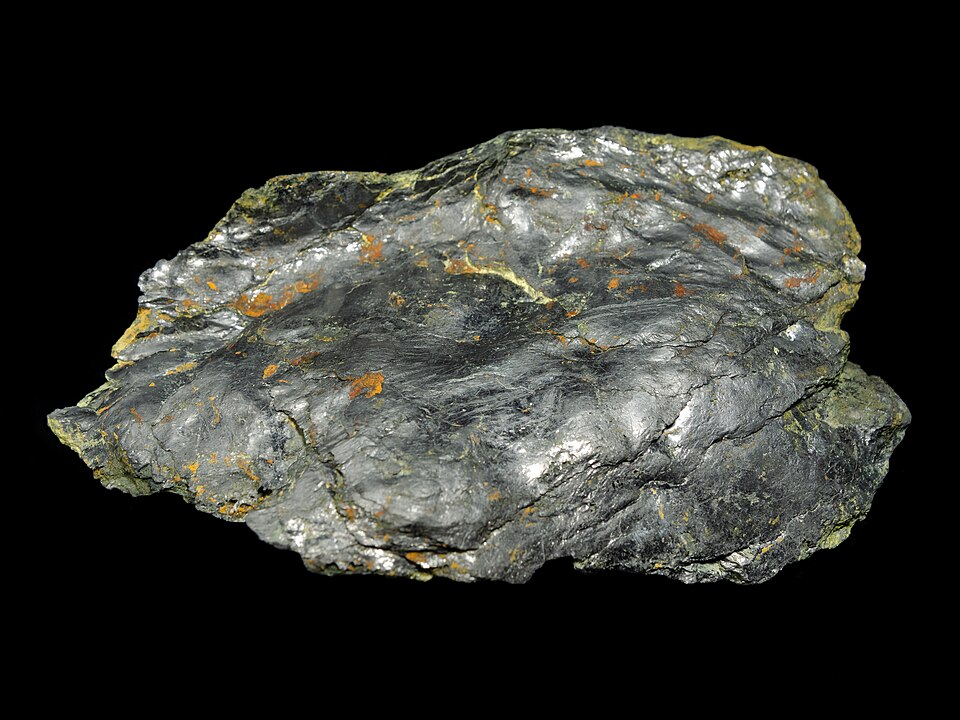
\includegraphics[width=0.36\linewidth]{images/book2/graphite.jpg}

{\small Un échantillon de graphite naturel, à l'éclat métallique.
Photo~: Zbynek Burival, CC BY-SA 4.0.}
\end{omfigure}

\section{Cristaux moléculaires}

\begin{definition}[Cristal moléculaire]\label{def:b1:crystals-ionic-covalent:molecular-crystal}
Un \emph{cristal moléculaire}\index{cristal moleculaire@cristal moléculaire} est un \omterm{def:b1:crystals-metals:crystal}{cristal} de
molécules maintenues ensemble par des interactions intermoléculaires ---
\omterm{def:b1:intermolecular-forces-solvents:vdw}{interactions de van der Waals} et, si possible, \omterm{def:b1:intermolecular-forces-solvents:hbond}{liaisons hydrogène} ---,
chaque molécule gardant ses propres \omterm{def:b1:lewis-resonance-vsepr:lewis}{liaisons covalentes}~: diiode, glace
carbonique \ce{CO2(s)}, glace, sucre.
\end{definition}

\begin{proposition}[Propriétés des cristaux moléculaires]\label{prop:b1:crystals-ionic-covalent:molecular}
Les \omterm{def:b1:crystals-ionic-covalent:molecular-crystal}{cristaux moléculaires} sont tendres et fondent ou se subliment à
basse température, puisque seules de faibles interactions
intermoléculaires sont rompues~; ils ne conduisent pas.
\end{proposition}
\admitted

\begin{example}[La glace]\label{ex:b1:crystals-ionic-covalent:ice}
Dans la glace ordinaire, chaque molécule d'eau est liée par \omterm{def:b1:intermolecular-forces-solvents:hbond}{liaison
hydrogène} à quatre autres situées aux sommets d'un tétraèdre~: deux par
ses propres hydrogènes et deux par ses \omterm{def:b1:lewis-resonance-vsepr:lewis}{doublets non liants}. Ce réseau
hexagonal ouvert, imposé par les directions des \omterm{def:b1:intermolecular-forces-solvents:hbond}{liaisons hydrogène},
laisse beaucoup de vide~: la glace est moins dense que l'eau liquide,
où le \omterm{def:b1:crystals-metals:lattice}{réseau} est en partie rompu et les molécules se rapprochent. La
symétrie hexagonale du réseau se lit dans la forme à six branches des
\omterm{def:b1:crystals-metals:crystal}{cristaux} de neige.
\end{example}

\begin{omfigure}
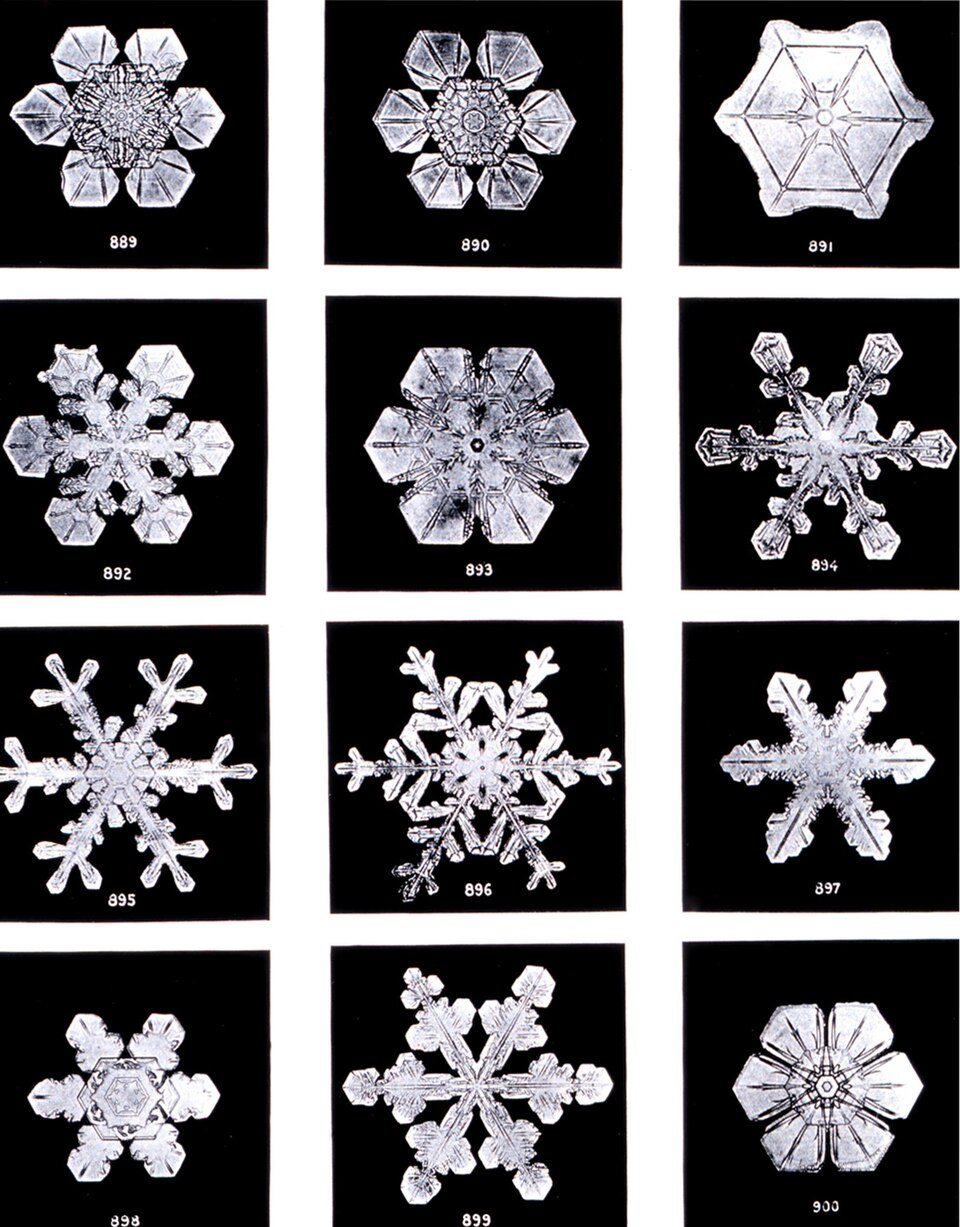
\includegraphics[width=0.38\linewidth]{images/book2/bentley-snowflakes.jpg}

{\small \omterm{def:b1:crystals-metals:crystal}{Cristaux} de neige photographiés par Wilson Bentley vers 1902~:
tous ont une symétrie d'ordre six, trace du réseau hexagonal de \omterm{def:b1:intermolecular-forces-solvents:hbond}{liaisons
hydrogène} de la glace. Domaine public.}
\end{omfigure}

\section{Comparaison des quatre sortes de solides}

\begin{center}
\small
\begin{tabular}{lllll}
\hline
solide & particules & cohésion & propriétés & exemples \\
\hline
métallique & cations, électrons & \omterm{def:b1:crystals-metals:metallic-bond}{liaison métallique} & conducteur, ductile & \ce{Cu}, \ce{Fe}, \ce{Na} \\
ionique & cations, anions & électrostatique & dur, cassant, isolant & \ce{NaCl}, \ce{CaF2} \\
covalent & atomes & \omterm{def:b1:lewis-resonance-vsepr:lewis}{liaisons covalentes} & très dur, fusion haute & diamant, \ce{SiO2} \\
moléculaire & molécules & van der Waals, liaisons H & tendre, fusion basse & \ce{I2}, glace \\
\hline
\end{tabular}
\end{center}

\begin{remark}[Un continuum]\label{rem:b1:crystals-ionic-covalent:continuum}
Les classes sont des idéalisations. Le sulfure de zinc a des liaisons en
partie ioniques, en partie covalentes, ce qui explique que sa distance
soufre--zinc soit plus courte que la somme des \omterm{def:b1:periodicity:radius}{rayons ioniques}~; le
graphite est covalent dans ses plans et moléculaire entre eux. La
différence d'\omterm{def:b1:periodicity:electronegativity}{électronégativité} (\cref{prop:b1:periodicity:en-trend}) est
le guide~: plus elle est grande, plus le solide est ionique.
\end{remark}

\section{Exercices}

\begin{exercise}[$\star$]\label{exo:b1:crystals-ionic-covalent:1}
Dans la \omterm{def:b1:crystals-metals:lattice}{maille} du sel gemme, dénombrer les cations et les anions, donner
la \omterm{def:b1:crystals-metals:coordination}{coordinence} de chacun et vérifier que la formule \ce{NaCl} est
respectée.
\end{exercise}

\begin{exercise}[$\star$]\label{exo:b1:crystals-ionic-covalent:2}
Le chlorure de césium a $a = \qty{412.3}{pm}$. Calculer la plus courte
distance \ce{Cs-Cl} et le nombre d'unités formulaires par \omterm{def:b1:crystals-metals:lattice}{maille}.
\end{exercise}

\begin{exercise}[$\star$]\label{exo:b1:crystals-ionic-covalent:3}
À l'aide des rayons $r(\ce{Na+}) = \qty{102}{pm}$ et $r(\ce{Cl-}) =
\qty{181}{pm}$, calculer le \omterm{def:b1:crystals-ionic-covalent:radius-ratio}{rapport des rayons} de \ce{NaCl} et prévoir la
\omterm{def:b1:crystals-metals:coordination}{coordinence} du cation.
\end{exercise}

\begin{exercise}[$\star$]\label{exo:b1:crystals-ionic-covalent:4}
Classer en solides métalliques, ioniques, covalents ou moléculaires~: le
cuivre, le chlorure de sodium, le diamant, le diiode, le quartz
\ce{SiO2}, la glace, le fluorure de calcium.
\end{exercise}

\begin{exercise}[$\star\star$]\label{exo:b1:crystals-ionic-covalent:5}
Démontrer que la structure sel gemme exige $r_+/r_- \ge \sqrt2 - 1$.
\end{exercise}

\begin{exercise}[$\star\star$]\label{exo:b1:crystals-ionic-covalent:6}
Calculer la masse volumique du chlorure de sodium à partir de
$a = \qty{564.1}{pm}$
($M(\ce{NaCl}) = \qty{58.44}{g/mol}$) et comparer à \qty{2.17}{g/cm^3}.
\end{exercise}

\begin{exercise}[$\star\star$]\label{exo:b1:crystals-ionic-covalent:7}
Calculer la masse volumique du chlorure de césium ($M = \qty{168.36}{g/mol}$,
$a = \qty{412.3}{pm}$) et comparer à la valeur mesurée, \qty{3.99}{g/cm^3}.
% ledger: rho:CsCl
\end{exercise}

\begin{exercise}[$\star\star$]\label{exo:b1:crystals-ionic-covalent:8}
Pour la blende ($a = \qty{540.9}{pm}$, $M = \qty{97.44}{g/mol}$),
calculer la distance \ce{Zn-S} et la masse volumique, et comparer à la
valeur mesurée, \qty{4.04}{g/cm^3}.
% ledger: rho:ZnS
\end{exercise}

\begin{exercise}[$\star\star$]\label{exo:b1:crystals-ionic-covalent:9}
Le graphite a une \omterm{def:b1:crystals-metals:lattice}{maille} hexagonale de paramètres $a = \qty{245.6}{pm}$
et $c = \qty{669.6}{pm}$, contenant 4 atomes. Calculer la distance
\ce{C-C} dans un plan ($a/\sqrt3$), la distance entre plans ($c/2$) et
la masse volumique. Pourquoi le graphite est-il moins dense que le
diamant~?
\end{exercise}

\begin{exercise}[$\star\star\star$]\label{exo:b1:crystals-ionic-covalent:10}
Démontrer que la \omterm{def:b1:crystals-metals:compactness}{compacité} du diamant vaut $\pi\sqrt3/16$, et expliquer
pourquoi le matériau le plus dur est l'un des moins compacts.
\end{exercise}

\begin{exercise}[$\star\star\star$]\label{exo:b1:crystals-ionic-covalent:11}
Le silicium a la structure diamant avec $a = \qty{543.1}{pm}$. Calculer
la longueur de la liaison \ce{Si-Si}, le \omterm{def:b1:periodicity:radius}{rayon covalent} du silicium et
la masse volumique ($M = \qty{28.09}{g/mol}$)~; comparer à
\qty{2.33}{g/cm^3}.
\end{exercise}

\begin{exercise}[$\star\star\star$]\label{exo:b1:crystals-ionic-covalent:12}
Pour le chlorure de rubidium, $r(\ce{Rb+}) = \qty{152}{pm}$ (six
voisins) et $r(\ce{Cl-}) = \qty{181}{pm}$. Quelle structure la règle du
\omterm{def:b1:crystals-ionic-covalent:radius-ratio}{rapport des rayons} prévoit-elle~? Dans les conditions ordinaires, il est
du \omterm{def:b1:crystals-ionic-covalent:structure-type}{type sel gemme} avec $a = \qty{658.1}{pm}$~: vérifier la distance
\ce{Rb-Cl}, et proposer une raison de l'échec de la règle.
% ledger: rion:Rb+VI, rion:Cl-VI, lat:RbCl
\end{exercise}

\section{Problème~: la fluorine, le minéral et la lentille}

\begin{problem}[{Problème du week-end --- la \omterm{def:b1:crystals-metals:lattice}{maille} de la fluorine, son
\omterm{def:b1:crystals-ionic-covalent:radius-ratio}{rapport des rayons}, deux parents (\ce{Li2O} et le diamant), et la masse
volumique de la fluorine calculée à partir de sa \omterm{def:b1:crystals-metals:lattice}{maille}}]
\label{pb:b1:crystals-ionic-covalent:1}
La fluorine, \ce{CaF2}, est un minéral~; obtenue en grands \omterm{def:b1:crystals-metals:crystal}{cristaux}
limpides, elle sert à faire des lentilles qui transmettent
l'ultraviolet. Sa \omterm{def:b1:crystals-metals:lattice}{maille} est cubique, $a =
\qty{546.3}{pm}$~; \ce{Ca^{2+}} sur un \omterm{def:b1:crystals-metals:lattice}{réseau} CFC, \ce{F-} dans les \omterm{def:b1:crystals-metals:site}{sites
tétraédriques}. Rayons~: $r(\ce{Ca^{2+}}) = \qty{112}{pm}$ (huit
voisins), $r(\ce{F-}) = \qty{131}{pm}$ (quatre voisins). Masses molaires
(g/mol)~: \ce{Ca} 40.08, \ce{F} 19.00, \ce{Li} 6.94, \ce{O} 16.00,
\ce{C} 12.01, \ce{Si} 28.09~; $N_A = \qty{6.022e23}{mol^{-1}}$.
% ledger: lat:CaF2, rion:Ca2+VIII, rion:F-IV, aw:Ca, aw:F, aw:Li, aw:O,
% aw:C, aw:Si, const:NA

\medskip
\noindent\textbf{Partie I --- La \omterm{def:b1:crystals-metals:lattice}{maille}.}
\begin{enumerate}
  \item Donner les positions des ions \ce{Ca^{2+}} dans la \omterm{def:b1:crystals-metals:lattice}{maille} et les
        dénombrer.
  \item Combien de \omterm{def:b1:crystals-metals:site}{sites tétraédriques} la \omterm{def:b1:crystals-metals:lattice}{maille} contient-elle~? En
        déduire le nombre d'ions \ce{F-} et vérifier la formule.
  \item Quelle est la \omterm{def:b1:crystals-metals:coordination}{coordinence} de \ce{F-}~? Celle de \ce{Ca^{2+}}~?
  \item Calculer la plus courte distance \ce{Ca-F}.
  \item La comparer à la somme des \omterm{def:b1:periodicity:radius}{rayons ioniques}.
  \item Calculer la plus courte distance \ce{F-F} et dire si les anions
        se touchent.
\end{enumerate}

\medskip
\noindent\textbf{Partie II --- Le \omterm{def:b1:crystals-ionic-covalent:radius-ratio}{rapport des rayons}.}
\begin{enumerate}[resume]
  \item Calculer $x = r_+/r_-$.
  \item Quelle \omterm{def:b1:crystals-metals:coordination}{coordinence} du cation la règle du \omterm{def:b1:crystals-ionic-covalent:radius-ratio}{rapport des rayons}
        permet-elle~?
  \item Pourquoi \ce{CaF2} ne peut-il pas adopter la structure du
        chlorure de césium, bien que son cation soit de \omterm{def:b1:crystals-metals:coordination}{coordinence} 8~?
  \item Décrire la fluorine comme un arrangement cubique simple d'ions
        \ce{F-}, avec des ions \ce{Ca^{2+}} au centre de la moitié des
        petits cubes.
  \item Calculer la \omterm{def:b1:crystals-metals:compactness}{compacité} de la fluorine.
\end{enumerate}

\medskip
\noindent\textbf{Partie III --- Deux parents.}
L'oxyde de lithium, \ce{Li2O}, est de \omterm{def:b1:crystals-ionic-covalent:structure-type}{type antifluorine} avec
$a = \qty{461.9}{pm}$~;
$r(\ce{Li+}) = \qty{59}{pm}$ (quatre voisins), $r(\ce{O^{2-}}) =
\qty{142}{pm}$ (huit voisins). Diamant~: $a = \qty{356.7}{pm}$.
% ledger: lat:Li2O, rion:Li+IV, rion:O2-VIII, rho:Li2O, lat:C-diamond
\begin{enumerate}[resume]
  \item Où se trouvent les ions \ce{O^{2-}} et \ce{Li+} dans la \omterm{def:b1:crystals-metals:lattice}{maille}
        antifluorine~?
  \item Calculer la distance \ce{Li-O} et la comparer à la somme des
        rayons.
  \item Calculer la masse volumique de \ce{Li2O} et la comparer à la
        valeur mesurée, \qty{2.01}{g/cm^3}.
  \item Quelle structure ionique a le même arrangement de positions que
        le diamant~?
  \item Calculer la longueur de la liaison \ce{C-C} et la masse
        volumique du diamant.
  \item Pourquoi le diamant est-il tellement moins compact que la
        fluorine, alors que ses atomes occupent le même type de
        positions~?
\end{enumerate}

\medskip
\noindent\textbf{Partie IV --- La masse volumique de la fluorine.}
\begin{enumerate}[resume]
  \item Calculer la masse molaire de \ce{CaF2}.
  \item Calculer la masse d'une \omterm{def:b1:crystals-metals:lattice}{maille}.
  \item Calculer le volume d'une \omterm{def:b1:crystals-metals:lattice}{maille}, en \unit{cm^3}.
  \item Quel serait l'effet sur la masse volumique d'une lacune sur un
        site \ce{F-} toutes les cent \omterm{def:b1:crystals-metals:lattice}{mailles}~?
  \item Calculer la masse volumique de la fluorine à partir de sa
        \omterm{def:b1:crystals-metals:lattice}{maille}, et la comparer à la valeur mesurée, \qty{3.18}{g/cm^3}.
\end{enumerate}
% ledger: rho:CaF2
\end{problem}
